\section{Experiments and Results}


\begin{table*}[t]
\centering
\caption{Controller parameters}
\label{tab:controller_param_table}
\begin{tabular}{lcccccc}
\hline\noalign{\smallskip}
                                                        &                       & \makecell{Synthetic\\Trials} 
                                                                                & \makecell{Rope\\Winding}
                                                                                & \makecell{Table\\Coverage}
                                                                                & \makecell{Two Stage\\Coverage} \\
\noalign{\smallskip}\hline\noalign{\smallskip}
\makecell[l]{$\tanse{3}$ inner\\product constant}      & $\rotvelweight$        &   - & 0.0025 & 0.0025 & 0.0025 \\
\noalign{\smallskip}
\makecell[l]{Servoing max\\gripper velocity}           & $\grippervelmaxservo$  & 0.1 &    0.2 &    0.2 &    0.2 \\
\noalign{\smallskip}
\makecell[l]{Obstacle avoidance\\max gripper velocity} & $\grippervelmaxobs$    &   - &    0.2 &    0.2 &    0.2 \\
\noalign{\smallskip}
\makecell[l]{Obstacle avoidance\\scale factor}         & $\obsavoidfactor$      &   - &    200 &   1000 &   1000 \\
\noalign{\smallskip}
\makecell[l]{Stretching correction\\scale factor}      & $\stretchweightfactor$ &   - &  0.005 &   0.03 &   0.03 \\
\hline
\end{tabular}
\end{table*}
\begin{table*}[t]
\centering
\caption{KF-MANB and KF-MANDB parameters}
\label{tab:param_table}
\begin{tabular}{lcccccc}
\hline\noalign{\smallskip}
                                                            &                               & \makecell{Synthetic\\Trials} 
                                                                                            & \makecell{Rope\\Winding}
                                                                                            & \makecell{Table\\Coverage}
                                                                                            & \makecell{Two Stage\\Coverage} \\
\noalign{\smallskip}\hline\noalign{\smallskip}
\makecell[l]{Correlation strength factor\\(KF-MANDB only)}  & $\correlationfactor$          &  0.9 &   0.9 &   0.9 &   0.9 \\
\noalign{\smallskip}
Transition noise factor                                     & $\transitionnoisefactor^2$    &    1 &   0.1 &   0.1 &   0.1 \\
\noalign{\smallskip}
Observation noise factor                                    & $\observationnoisefactor^2$   &    1 &  0.01 &  0.01 &  0.01 \\
\noalign{\smallskip}\hline
\end{tabular}
\end{table*}

We test our method on three synthetic tests and three deformable object manipulation tasks in simulation. The synthetic tasks show that the principles we use to estimate the coupling between models are reasonable; while the simulated tasks show that our method is effective at performing deformable object manipulation tasks. Table~\ref{tab:controller_param_table} shows the parameters used by the Jacobian-based controller, while Table~\ref{tab:param_table} shows the parameters used by the the bandit algorithms for all experiments. We chose these parameters by comparing performance across noise factors $\observationnoisefactor^2$ and $\transitionnoisefactor^2$ from $\{0.01, 0.1, 1, 10\}$ and correlation strength factor $\correlationfactor$ from $\{0.1, 0.5, 0.9, 0.99\}$. While performance on individual experiments could be marginally improved by using different values, we found that $\observationnoisefactor^2=0.01$, $\transitionnoisefactor^2=0.1$, and $\correlationfactor=0.9$ resulted in robust performance for all of our manipulation tasks. $\utilityprocessscale$ is set dynamically and discussed in Sec.~\ref{sec:synthetic_trials}.




\subsection{Synthetic Tests}
\label{sec:synthetic_trials}


For the synthetic tests, we set up an underactuated system that is representative of manipulating a deformable object with configuration $y \in \reals^n$ and control input $\dot x \in \reals^m$ such that $m < n$ and $\dot y = J \dot x$. To construct the Jacobian of this system we start with $J = \begin{bmatrix}\eye_{m \times m} \\ \mathbf{0}_{(n-m) \times m} \end{bmatrix}$ and add uniform noise drawn from $[-0.1, 0.1]$ to each element of $J$. The system configuration starts at $\begin{bmatrix}10 & \dots & 10\end{bmatrix}^T$ with the target configuration set to the origin. Error is defined as $\ErrorFn(t) = \| y(t) \|$, and the desired direction to move the system at each timestep is $\dot y_d(t) = - y(t)$. These tasks have no obstacles or stretching, thus $\obsavoidfactor, \stretchweightfactor,$ and $\grippervelmaxobs$ are unused. Rather than setting the utility noise scale $\utilityprocessscale$ \textit{a priori}, we use an annealing filter
\begin{equation}
    \utilityprocessscale(t+1) = \max(10^{-10}, 0.9 \utilityprocessscale(t) + 0.1 |\reward(t+1)|) \enspace.
\end{equation}
This enables us to track the changing available reward as the system gets closer to the target.

To generate a model for the model set we start with the true Jacobian $J$ and add uniform noise drawn from $[-0.025, 0.025]$ to each element of $J$. For an individual trial, each bandit algorithm uses the same $J$ and the same model set. Each bandit algorithm receives the same random number stream during a trial, ensuring that a more favourable stream doesn't bias results. We ran one small test using a $3 \times 2$ Jacobian with 10 arms in order to yield results that are easily visualised. The second and third tests are representative of the scale of the simulation experiments, using the same number of models and similar sizes of Jacobian as are used in simulation. A single trial consists of 1000 pulls (1000 commanded actions); each test was performed 100 times to generate statistically significant results. Our results in Table~\ref{tab:synthetic_results} show that KF-MANDB clearly performs the best for all three tests.


\begin{table}[ht]
\centering
\caption{Synthetic trial results showing total regret with standard deviation in brackets for all bandit algorithms for 100 runs of each setup.}
\label{tab:synthetic_results}
\begin{tabular}{cccccc}
\hline\noalign{\smallskip}
\makecell{\# of\\Models} & \makecell{\# of rows\\in $J$}    & \makecell{\# of cols\\in $J$} & UCB1-Normal & KF-MANB     & KF-MANDB \\
\noalign{\smallskip}\hline\noalign{\smallskip}
10                      & 3                                 & 2                             & 4.41 [1.65] & 3.62 [1.73] & 2.99 [1.40] \\
60                      & 147                               & 6                             & 5.57 [1.37] & 4.89 [1.32] & 4.53 [1.42] \\
60                      & 6075                              & 12                            & 4.21 [0.64] & 3.30 [0.56] & 2.56 [0.54] \\
\hline
\end{tabular}
\end{table}


\subsection{Simulation Trials}

\begin{figure*}[t]
    \centering
    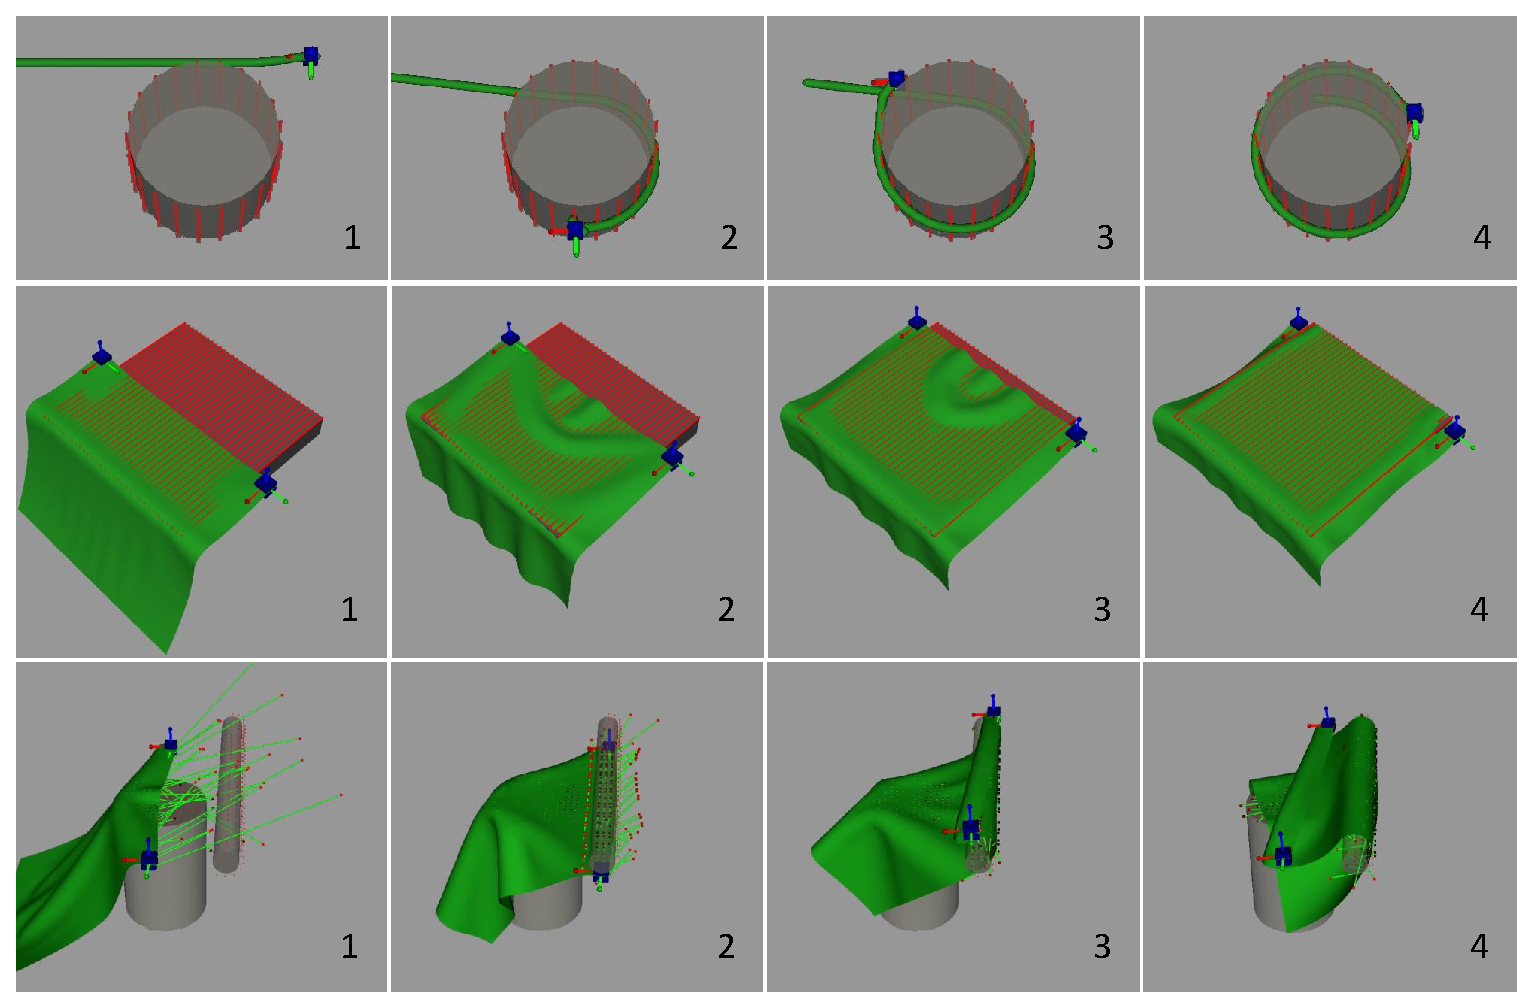
\includegraphics[width=\textwidth]{CombinedImages}
    \caption{Sequence of snapshots showing the execution of the simulated experiments using the KF-MANDB algorithm. The rope and cloth are shown in green, the grippers is shown in blue, and the target points are shown in red. The bottom row additionally shows $\deformvel_d$ as green rays with red tips.}
    \label{fig:simulation_task_screenshots}
\end{figure*}


We now demonstrate the effectiveness of multi-arm bandit techniques on three example tasks, show how to encode those tasks for use in our framework, and discuss experimental results. The first task shows how our method can be applied to a rope, with the goal of winding the rope around a cylinder in the environment. The second and third tasks show the method applied to cloth. In the second task, two grippers manipulate the cloth so that it covers a table. In the third task, we perform a two-stage coverage task, covering portions of two different cylinders. In all three tasks, the alignment error $\ErrorFn(\deformconfig, \target)$ is measured as the sum of the distances between every point in $\target$ and the closest point in $\deformconfig$ in meters. Figure~\ref{fig:simulation_task_screenshots} shows the target points in red, and the deformable object in green. The video accompanying this paper shows the task executions.

All experiments were conducted in the open-source Bullet simulator~\cite{Coumans2010}, with additional wrapper code developed at UC Berkeley. The rope is modeled as a series of 49 small capsules linked together by springs and is 1.225m long. The cloth is modeled as a triangle mesh of size $0.5\text{m} \times 0.5\text{m}$ for the table coverage task, and size $0.5\text{m} \times 0.625\text{m}$ for the two-stage coverage task. We emphasize that our method does not have access to the model of the deformable object or the simulation parameters. The simulator is used as a ``black box'' for testing.\footnote{Our code is available at \url{https://github.com/UM-ARM-Lab/mab_ms}.}

In addition to the diminishing rigidity model introduced in Section~\ref{sec:diminishing_rigidity} we will also use \textit{adaptive Jacobian} models based on the work of \citet{Navarro-Alarcon2014}. This formulation uses an online estimation method to approximate $\Jacobian(\gripperconfig, \deformconfig)$.
First we with some estimate of the Jacobian $\tilde \Jacobian(0)$ at time $t = 0$ and then use the Broyden update rule~\cite{Broyden1965} to update $\tilde \Jacobian(t)$ at each timestep $t$
\begin{equation}
    \tilde \Jacobian(t) = \tilde J(t-1) + \ajrate \frac{\left( \deformvel(t) - \tilde \Jacobian(t-1) \grippervel(t) \right)}{\grippervel(t)^T \grippervel(t)} \grippervel(t)^T \enspace.
\end{equation}
This update rule depends on a update rate $\ajrate \in (0, 1]$ which controls how quickly the estimate shifts between timesteps.

We use models generated using the same parameters for all three tasks with a total of 60 models: 49 diminishing rigidity models with rotation and translational deformability values $\drktrans$ and $\drkrot$ ranging from 0 to 24 in steps of 4, as well as 11 adaptive Jacobian models with learning rates $\ajrate$ ranging from $1$ to $10^{-10}$ in multiples of 10. All adaptive Jacobian models are initialized with the same starting values; we use the diminishing rigidity Jacobian for this seed with $\drktrans=\drkrot=10$ for the rope experiment and $\drktrans=\drkrot=14$ for the cloth experiments to match the best model found in~\cite{Berenson2013}. We use the same strategy for setting $\utilityprocessscale$ as we use for the synthetic tests. 
%App~\ref{apx:param_table} shows all other parameters.

We evaluate results for the MAB algorithms as well as using each of the models in the set for the entire task. To calculate regret for each MAB algorithm, we create copies of the simulator at every timestep and simulate the gripper command, then measure the resulting reward $\reward_\modelidx(t)$ for each model. The reward of the best model $\reward^*(t)$ is then the maximum of individual rewards. As KF-MANB and KF-MANDB are not deterministic algorithms, each task is performed 10 times for these methods. All tests are run on an Intel Xeon E5-2683 v4 processor with 64 GB of RAM. UCB1-Normal and KF-MANB solve Eq.~\eqref{eqn:jacobianbackwardfunction_sim} once per timestep, while KF-MANDB solves it for every model in $\modelset$. Computation times for each test are shown in their respective sections.


\textit{Winding a Rope Around a Cylinder}: In the first example task, a single gripper holds a rope that is lying on a table. The task is to wind the rope around a cylinder which is also on the table (see Fig.~\ref{fig:simulation_task_screenshots}). Our results~(Fig.~\ref{fig:ropecylinder_results}) show that at the start of the task all the individual models perform nearly identically, starting to split at 2 seconds (when the gripper first approaches the cylinder) and again at 6 seconds. Despite our model set containing models that are unable to perform the task, our formulation is able to successfully perform the task using all three bandit algorithms. Interestingly, while KF-MANDB outperforms UCB1-Normal and KF-MANB in terms of regret, all three algorithms produce very similar results. Solving Eq.~\eqref{eqn:jacobianbackwardfunction_sim} at each iteration requires an average of 17.3~ms (std. dev. 5.5~ms) for a single model, and 239.5~ms (std. dev. 153.7~ms) for 60 models.


\begin{figure*}[t]
    \centering
    \vspace{-0.1in}
    \subfloat{
        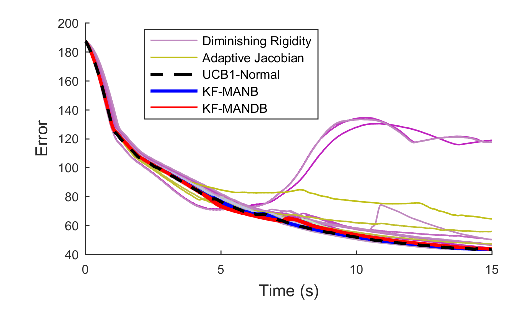
\includegraphics[width=0.45\textwidth]{rope_cylinder_wafr_tase_submission_error}
    }
    \subfloat{
        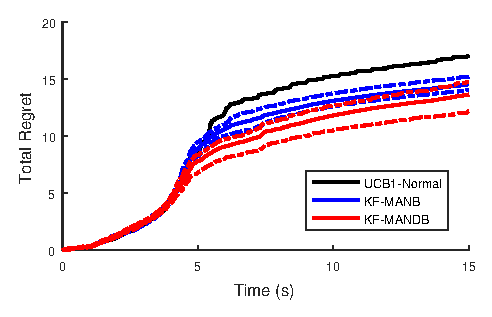
\includegraphics[width=0.45\textwidth]{rope_cylinder_wafr_tase_submission_total_regret}
    }
    \\
    \vspace{-0.15in}
    \subfloat{
        \hspace{-0.1in}
        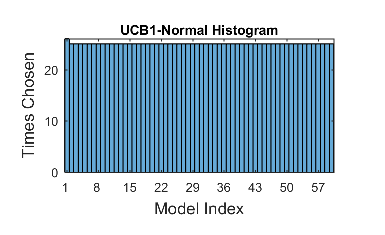
\includegraphics[width=0.35\textwidth]{rope_cylinder_wafr_tase_submission_UCB_histogram}
        \hspace{-0.25in}
    }
    \subfloat{
        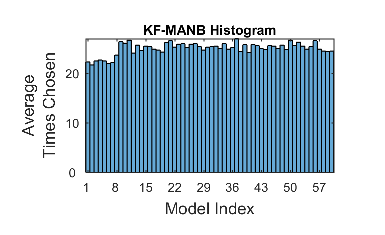
\includegraphics[width=0.35\textwidth]{rope_cylinder_wafr_tase_submission_KFMANB_histogram}
    }
    \subfloat{
        \hspace{-0.25in}
        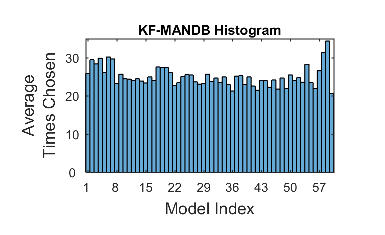
\includegraphics[width=0.35\textwidth]{rope_cylinder_wafr_tase_submission_KFMANDB_histogram}
        \hspace{-0.1in}
    }
    \vspace{-0.1in}
    \caption{Experimental results for the rope-winding task. Top left: alignment error for 10 trials for each MAB algorithm, and each model in the model set when used in isolation. UCB1-Normal, KF-MANB, KF-MANDB lines overlap in the figure for all trials. Top right: Total regret averaged across 10 trials for each MAB algorithm with the minimum and maximum drawn in dashed lines. Bottom row: histograms of the number of times each model was selected by each MAB algorithm; UCB1-Normal (bl), KF-MANB (bm), KF-MANDB (br).}
    \label{fig:ropecylinder_results}
\end{figure*}



\textit{Spreading a Cloth Across a Table}: The second scenario we consider is spreading a cloth across a table. In this scenario two grippers hold the rectangular cloth at two corners and the task is to cover the top of the table with the cloth. All of the models are able to perform the task (see Fig.~\ref{fig:clothtable_results}), however, many single-model runs are slower than the bandit methods at completing the task, showing the advantage of the bandit methods. When comparing between the bandit methods, both error and total regret indicate no performance difference between the methods. Solving Eq.~\eqref{eqn:jacobianbackwardfunction_sim} at each iteration requires an average of 89.5~ms (std. dev. 82.4~ms) for a single model, and 605.1~ms (std. dev. 514.3~ms) for 60 models.


\begin{figure*}[t]
    \centering
    \vspace{-0.1in}
    \subfloat{
        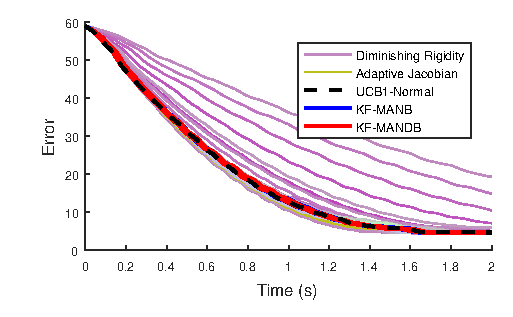
\includegraphics[width=0.45\textwidth]{cloth_table_wafr_tase_submission_error}
    }
    \subfloat{
        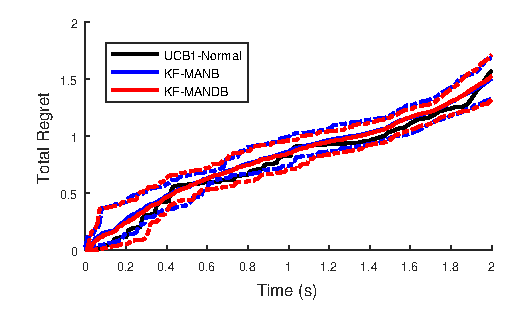
\includegraphics[width=0.45\textwidth]{cloth_table_wafr_tase_submission_total_regret}
    }
    \\
    \vspace{-0.15in}
    \subfloat{
        \hspace{-0.1in}
        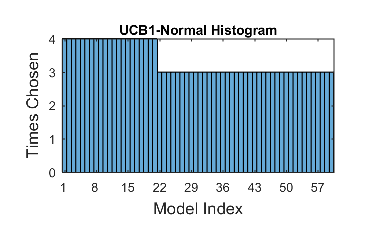
\includegraphics[width=0.35\textwidth]{cloth_table_wafr_tase_submission_UCB_histogram}
        \hspace{-0.25in}
    }
    \subfloat{
        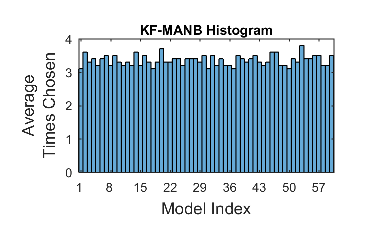
\includegraphics[width=0.35\textwidth]{cloth_table_wafr_tase_submission_KFMANB_histogram}
    }
    \subfloat{
        \hspace{-0.25in}
        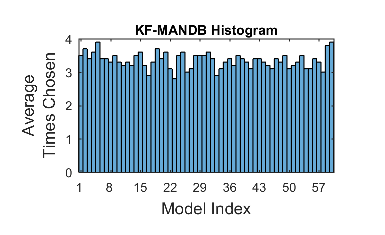
\includegraphics[width=0.35\textwidth]{cloth_table_wafr_tase_submission_KFMANDB_histogram}
        \hspace{-0.1in}
    }
    \vspace{-0.1in}
    \caption{Experimental results for the table coverage task. See Fig.~\ref{fig:ropecylinder_results} for description.}
    \label{fig:clothtable_results}
\end{figure*}



\textit{Two-Part Coverage Task}: In this experiment, we consider a two-part task. The first part of the task is to cover the top of a cylinder similar to our second scenario. The second part of the task is to cover the far side of a second cylinder. For this task the \texttt{GetTargets} function used previously pulls the cloth directly into the second cylinder. The collision avoidance term then negates any motion in that direction causing the grippers to stop moving. To deal with this, we discretize the free space using a voxel grid, and then use Dijkstra's algorithm to find a collision free path between each cover point and every point in free space. We use the result from Dijkstra's algorithm to define a vector field that pulls the nearest (as defined by Dijkstra's) deformable object point $p_k$ along the shortest collision free path to the target point. This task is the most complex of the three (see Fig.~\ref{fig:clothwafr_results}); many models are unable to perform the task at all, becoming stuck early in the task. We also observe that both KF-MANB and KF-MANDB show a preference for some models over others. Two interesting trials using KF-MANDB stand out; in the first the grippers end up on opposite sides of the second cylinder, in this configuration the physics engine has difficulty resolving the scene and allows the cloth to be pulled straight through the second cylinder. In the other trial the cloth is pulled off of the first cylinder, however KF-MANDB is able to recover, moving the cloth back onto the first cylinder. KF-MANDB and UCB1-Normal are able to perform the task significantly faster than KF-MANB, though all MAB methods complete the task using our formulation. Solving Eq.~\eqref{eqn:jacobianbackwardfunction_sim} at each iteration requires an average of 102.6~ms (std. dev. 30.6~ms) for a single model, and 565.5~ms (std. dev. 389.8~ms) for 60 models.


\begin{figure*}[t]
    \centering
    \subfloat{
        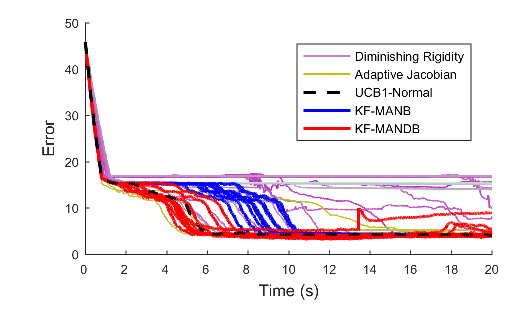
\includegraphics[width=0.45\textwidth]{cloth_wafr_wafr_tase_submission_error}
    }
    \subfloat{
        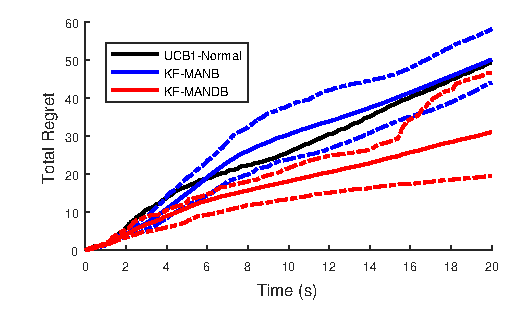
\includegraphics[width=0.45\textwidth]{cloth_wafr_wafr_tase_submission_total_regret}
    }
    \\
    \vspace{-0.15in}
    \subfloat{
        \hspace{-0.1in}
        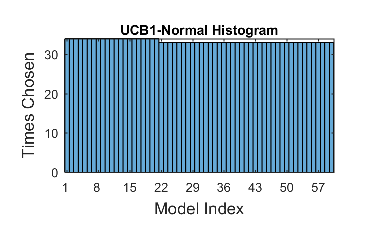
\includegraphics[width=0.35\textwidth]{cloth_wafr_wafr_tase_submission_UCB_histogram}
        \hspace{-0.25in}
    }
    \subfloat{
        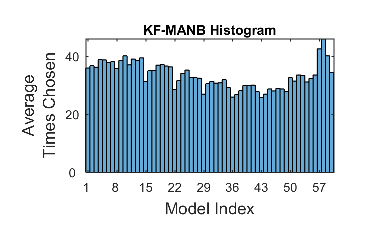
\includegraphics[width=0.35\textwidth]{cloth_wafr_wafr_tase_submission_KFMANB_histogram}
    }
    \subfloat{
        \hspace{-0.25in}
        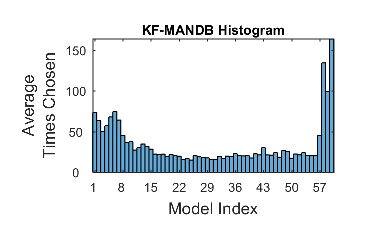
\includegraphics[width=0.35\textwidth]{cloth_wafr_wafr_tase_submission_KFMANDB_histogram}
        \hspace{-0.1in}
    }
    \vspace{-0.1in}
    \caption{Experimental results for the two-part coverage task. See Fig.~\ref{fig:ropecylinder_results} for description.}
    \label{fig:clothwafr_results}
\end{figure*}

\todoin{Add real robot example on Victor}